\documentclass{article}
\usepackage{amsmath, amssymb, amsthm}
\usepackage{inputenc}
\usepackage{geometry}
\usepackage{tikz}
\usepackage{multicol}
\usetikzlibrary{decorations.pathreplacing}
\geometry{legalpaper, portrait, margin=1in}
\begin{document}
APHY250

Exam I Study Sheet

Dylan VanAllen 

\section*{Waves and Vibrations}
\begin{itemize}
    \item The three forms to describe a wave. (1) is general, (2) and (3) are when \(C'=C*\): 
    \begin{align}
        \psi & = Ce^{i\omega t}+C'e^{-i\omega t} \\
        \psi & = A\cos{(\omega t)}+B\sin{(\omega t)} \\
        \psi & = A\cos{(\omega t+\phi)}
    \end{align}
    \item Since \(\psi\) represents displacement, \(\dot{\psi}\) is the velocity and has 
    an amplitude of \(\omega A\) and \(\ddot{\psi}\) is the acceleration and has 
    amplitude \(\omega^2 A\). \par \noindent
    \item The phase velocity of a wave is \(v_\phi = \frac{\omega}{k}\).
    \item A standing wave is described by \(\psi = 2A\cos{(kx)}\cos{(\omega t)}\). 
    The nodes of a standing wave are at \(x = \frac{(2n-1)\lambda}{4}\).
\end{itemize}

\section*{Free Vibrations}
\begin{itemize}
    \item The motion of a free vibarator is given by \(\ddot{\psi} + \frac{s}{m}\psi=0\), and  
    \(\omega_0^2 = \frac{s}{m}\). \(\omega_0\) is the angular frequency of the wave. The period 
    is \(T=\frac{2\pi}{\omega_0}\).
    \item The kinetic energy of a system can be modeled by 
    \begin{equation*}
        T = \frac{1}{2}m\dot{\psi}^2 = \frac{1}{2}m\omega_0^2 A^2 \sin(\omega_0 t + \phi)
    \end{equation*}
    Similarly the potential energy is
    \begin{equation*}
        V = \frac{1}{2}s\psi^2 = \frac{1}{2}m\omega_0^2 A^2 \cos^2(\omega_0 t + \phi)
    \end{equation*}
    The total energy is therefore \(W = T+V = \frac{1}{2}sA^2\) (constant).
    \par \noindent
    \item A pendulum's motion is modeled by \(\ddot{\psi}+\frac{g}{\ell}\sin\psi=0\).
    In this scenario, \(\psi\) is the angle from the vertical to the pendulum 
    and the angular frequency is \(\omega_0 = \sqrt{\frac{g}{\ell}}\).    
    \item A circuit oscillation can be given by \(\ddot{\psi}+\frac{1}{LC}\psi = 0\) where \(\psi\) 
    is the charge, and therefore \(\dot{\psi}\) is the current. \(L\) is the inductance and 
    \(C\) is the capacitance. Here, \(\omega_0 = \sqrt{\frac{1}{LC}}\).
\end{itemize}

\section*{Damping}
\begin{itemize}
    \item A dampened motion oscillator follows \(\ddot{\psi}+\gamma\dot{\psi}+\omega_0^2\psi=0\). Here, 
    \(\gamma = \frac{b}{m}\) where \(b\) is resistance. 
    \item Now the angular frequency is
    \begin{equation*} 
        \omega_f = \omega_0\sqrt{1-\left(\frac{\gamma}{2\omega_0}\right)^2} 
    \end{equation*}
    \item In light damping, \(\gamma < 2\omega_0\). Now \(\psi(t) = Ae^{-\frac{\gamma}{2}t}\cos(\omega_f t + \phi)\).
    Here the amplitude decays over time. Now \(\langle W\rangle = \frac{1}{2}m\omega_0^2 A^2 e^{-\gamma t}\).
    The fractional rate of energy loss is \(-\frac{1}{\langle W\rangle} \frac{d\langle W\rangle}{dt} \approx \gamma\).
    The time between successive zeros is \(\tau \equiv \frac{2\pi}{\omega_f}\). 
    \item  \(Q \equiv \frac{\omega_0}{\gamma}\). 
    \begin{equation*}
        Q \ \begin{cases}
            > \frac{1}{2} &\text{for light damping} \\
            = \frac{1}{2} &\text{for critical damping} \\
            < \frac{1}{2} &\text{for heavy damping}
        \end{cases}
    \end{equation*}
    \item In critical damping \(\gamma = 2\omega_0\), so \(\psi(t) = e^{-\omega_0 t}(c_1+c_2'\omega_0 t)\). 
    \item In heavy damping \(\gamma > 2\omega_0\), so \(\psi(t) = c_1 e^{-\mu_1 t}+c_2 e^{-\mu_2 t}\). Both \(\mu_1\) and 
    \(\mu_2\) are real and positive. \(\mu_1 > \mu_2\) and \(\mu_1 \mu_2 = \omega_0^2\).
    \item In resistance damping, the equation of charge oscillation is 
    \begin{equation*}
        \ddot{\psi} + \frac{R}{L}\dot{\psi} +\frac{1}{LC}\psi = 0
    \end{equation*}
    The analogy to motion is that \(L = m\), \(b=R\), and \(s = \frac{1}{C}\). 
\end{itemize}
\section*{Forced Vibrations}
\begin{itemize}
    \item The equation for forced vibrations is 
    \begin{equation*}
        \ddot{\psi} + \gamma\dot{\psi}+\omega_0^2\psi = \frac{F_0}{m}\cos(\omega t)
    \end{equation*}
    \item The solution is \(\psi = A\cos(\omega t + \phi)\), where \(\omega\) is the 'driving
    frequency'. At resonance, \(\omega = \omega_0\). The angle \(\phi\) is the angle formed on the vector diagram between the 
    sides \(\frac{F_0}{m}\) and \(\omega_0^2 A\). 
    \begin{equation*}
        |\sin\phi| = \sqrt{\frac{\gamma^2\omega^2}{(\omega_0^2-\omega^2)^2+\gamma^2\omega^2}}
    \end{equation*}
    \item The amplitude of displacement is \(A = \frac{F_0}{m\gamma\omega}|\sin\phi|\).
    \item Power absorption is given by: 
    \begin{equation*}
        \langle P \rangle = \frac{F_0^2}{2b}\left(\frac{\gamma^2\omega^2}{(\omega_0^2-\omega^2)^2+\gamma^2\omega^2}\right)
    \end{equation*}
    \item Vector diagrams for forced oscillations looks like this: 
\end{itemize}

\begin{multicols}{3}
\noindent

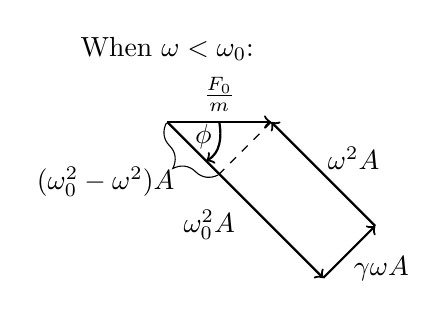
\begin{tikzpicture}[scale=0.33]
    \draw (0,8) node[anchor=south] {When \(\omega < \omega_0\):};
    \draw[thick,->] (0,6) -- (4,6) node[pos=0.5,anchor=south] {\(\frac{F_0}{m}\)} 
    node[pos=0.5,xshift=1pt,yshift=3pt, anchor=north east] {\(\phi\)};
    \draw[thick,->] (0,6) -- (6,0) node[pos=0.5,anchor=north east] {\(\omega_0^2 A\)};
    \draw[thick,->] (6,0) -- (8,2) node[pos=0.5, xshift=-2pt,yshift=2pt,anchor=north west] {\(\gamma\omega A\)};
    \draw[thick,->] (8,2) -- (4,6) node[pos=0.5, xshift=-2pt,yshift=-2pt,anchor=south west] {\(\omega^2 A\)};
    \draw[dashed] (4,6) -- (2,4);
    \draw[decorate, decoration={brace, amplitude=10pt}, xshift=-1pt,yshift=-1pt] (2,4) -- (0,6) 
    node[pos=0.5,xshift=-3pt,yshift=-3pt,anchor=north east] {\((\omega_0^2-\omega^2)A\)};
    \draw[thick,->] (2,6) to [out=-80,in=30] (1.5,4.5);
\end{tikzpicture}

\par \noindent
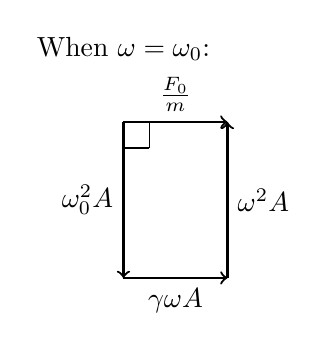
\begin{tikzpicture}[scale=0.33]
    \draw (0,8) node[anchor=south] {When \(\omega = \omega_0\):};
    \draw[thick,->] (0,6) -- (4,6) node[pos=0.5,anchor=south] {\(\frac{F_0}{m}\)};
    \draw[thick,->] (0,6) -- (0,0) node[pos=0.5,anchor=east] {\(\omega_0^2 A\)};
    \draw[thick,->] (0,0) -- (4,0) node[pos=0.5, anchor=north] {\(\gamma\omega A\)};
    \draw[thick,->] (4,0) -- (4,6) node[pos=0.5, anchor=west] {\(\omega^2 A\)};
    \draw (1,6) -- (1,5);
    \draw (0,5) -- (1,5);
\end{tikzpicture}
\par \noindent
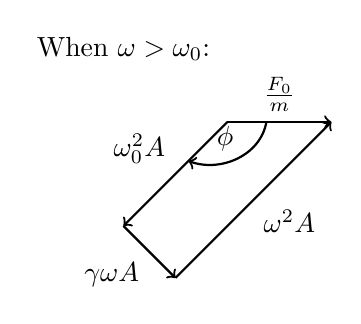
\begin{tikzpicture}[scale=0.33]
    \draw (0,8) node[anchor=south] {When \(\omega > \omega_0\):};
    \draw[thick,->] (4,6) -- (8,6) node[pos=0.5,anchor=south] {\(\frac{F_0}{m}\)};
    \draw[thick,->] (4,6) -- (0,2) node[pos=0.5,anchor=south east] {\(\omega_0^2 A\)};
    \draw[thick,->] (0,2) -- (2,0) node[pos=0.5, anchor=north east] {\(\gamma\omega A\)};
    \draw[thick,->] (2,0) -- (8,6) node[pos=0.5, anchor=north west] {\(\omega^2 A\)};
    \draw[thick,->] (5.5,6) to [out=-100,in=-20] (2.5,4.5) node[anchor=south east,xshift=20pt] {\(\phi\)};
\end{tikzpicture}
\end{multicols}
\end{document}
